%%%%%%%%%%%%%%%%%%%%%%%%%%%%%%%%%%%%%%%%%%%%%%%%%%
\begin{frame}{Überblick über die Präsentation}

\Large{Specification by Example}

\vspace{2em}

\begin{itemize}
	\item Motivation

	\item Ziel

	\item Weg

	\item Beispiel
\end{itemize}

\end{frame}


%%%%%%%%%%%%%%%%%%%%%%%%%%%%%%%%%%%%%%%%%%%%%%%%%%
\begin{frame}{Software aus verschiedenen Perspektiven}

\begin{itemize}

	
	\item Auftraggeber:

	\begin{itemize}
		\item \glqq Die Software soll tun, was ich erwarte.\grqq
		\item \glqq Ich will das Ganze möglichst preiswert.\grqq
	\end{itemize}
	
	
	\item Entwickler:
	
	\begin{itemize}
		\item \glqq Ich will wissen, was ich entwickeln soll.\grqq
		\item \glqq Wann bin ich fertig?\grqq
	\end{itemize}
	
	
	\item Nach der Lieferung:
	
	\begin{itemize}
		\item \glqq Was macht die Software genau?\grqq
		\item \glqq Bug oder Feature?\grqq
	\end{itemize}
\end{itemize}

\end{frame}


%%%%%%%%%%%%%%%%%%%%%%%%%%%%%%%%%%%%%%%%%%%%%%%%%%
\begin{frame}{Die Vision -- Eine Quelle für alle}

\begin{itemize}
	\item Beschreibung der Anforderung

	\item Akzeptanztests für die Entwicklung

	\item Ausführbare Dokumentation
\end{itemize}

\vspace{1em}

$\Rightarrow$ Single Source of Truth

\end{frame}


%%%%%%%%%%%%%%%%%%%%%%%%%%%%%%%%%%%%%%%%%%%%%%%%%%
\begin{frame}{Wie wir dahin kommen}


\begin{itemize}
	\item Kommunikation und Diskussion \em aller \em Beteiligten 
	
	\item Fokus auf die Fachlichkeit
\end{itemize}


\vspace{1em}

$\Rightarrow$ Specification Workshops

\end{frame}



%%%%%%%%%%%%%%%%%%%%%%%%%%%%%%%%%%%%%%%%%%%%%%%%%%
\begin{frame}{So kann ein Specification Workshop ablaufen}

\begin{itemize}
	\item Der Auftraggeber beschreibt sein zu lösendes Problem
	\item Die anderen Teilnehmer befragen ihn, um Klarheit zu erhalten
	\item Alle erarbeiten gemeinsam Beispiele
	\item Die Beispiele werden zusammengeführt und auf das Wesentliche reduziert
	\item Aus den Beispielen wird die ihnen zugrundeliegende Spezifikation abgeleitet
\end{itemize}

\end{frame}



%%%%%%%%%%%%%%%%%%%%%%%%%%%%%%%%%%%%%%%%%%%%%%%%%%
\begin{frame}{Darauf sollte man achten}

\begin{itemize}
   \item Komplizierte Beispiele
   
   \item Namensgebung
   
   \item Formeln
   
   \item Bei vielen Teilnehmern: Erstellung der Beispiele in Kleingruppen
\end{itemize}


\end{frame}



%%%%%%%%%%%%%%%%%%%%%%%%%%%%%%%%%%%%%%%%%%%%%%%%%%
\begin{frame}{Von den Beispielen hin zur Spezifikation}

\begin{itemize}
	\item Aus den Beispielen wird die Spezifikation abgeleitet (Zusammenfassung)
        \item Spezifikation wird gegen die Eingangsfragen geprüft
	\item Dadurch kann man die Vollständigkeit in beide Richtungen prüfen
	\item Muss auch von jemand verstanden werden, der nicht am Workshop teilgenommen hat
\end{itemize}

\end{frame}
 
%%%%%%%%%%%%%%%%%%%%%%%%%%%%%%%%%%%%%%%%%%%%%%%%%%
\begin{frame}{Beispiel: Konkrete Anforderung}

\begin{itemize}
	\item Ich bin Inhaber eines Hot Dog Standes und habe schon ein kleines Kassensystem mit Bestandsverwaltung
	\item Ich möchte, dass das System automatisch Nachschub bestellt, wenn mir die Würstchen ausgehen
	
	\item Was ich schon weiss:
	\begin{itemize}
		\item Mein Lieferant braucht maximal 30 Minuten
		\item Dienstags verkaufe ich mehr Würstchen
		\item Nach 16:00 Uhr verkaufe ich nicht mehr viel
	\end{itemize}
	
	\item So bestelle ich aktuell:
	\begin{itemize}
		\item Wenn der Bestand auf 10 Würstchen sinkt (Dienstags: 20)
		\item Nur vor 16:00 Uhr
	\end{itemize}
\end{itemize}
	
$\Rightarrow$ Bitte erstellt in kleinen Gruppen (ca. 4 Personen) Beispiele!

\end{frame}


%%%%%%%%%%%%%%%%%%%%%%%%%%%%%%%%%%%%%%%%%%%%%%%%%%
\begin{frame}{Möglichkeit 1}

\begin{center}
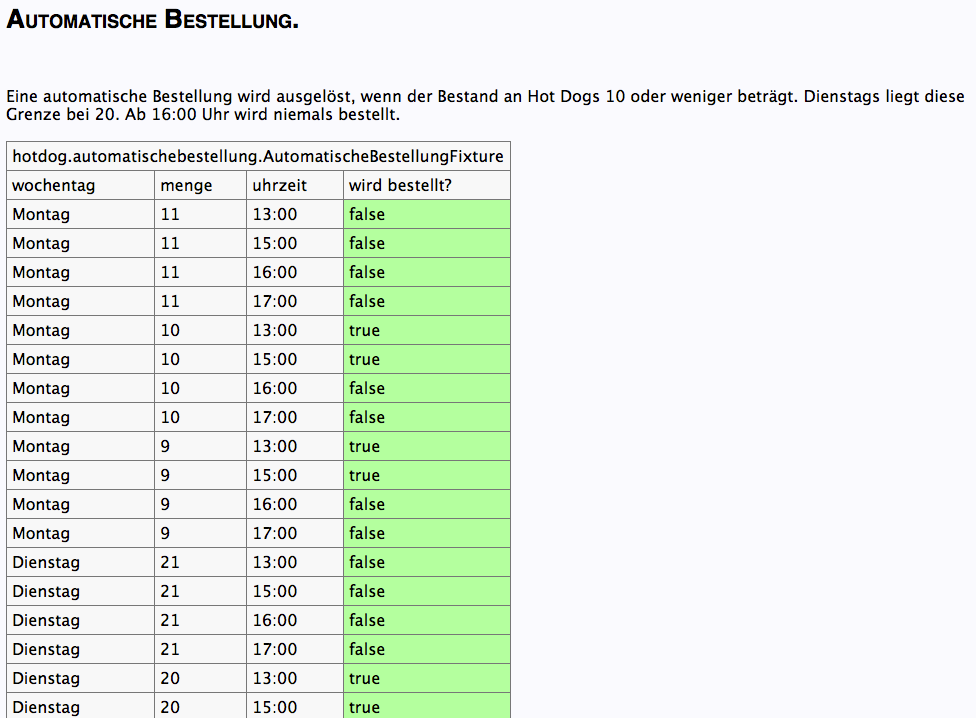
\includegraphics[height=7cm]{SchlechtesBeispiel.png} \newline
\end{center}

\end{frame}

%%%%%%%%%%%%%%%%%%%%%%%%%%%%%%%%%%%%%%%%%%%%%%%%%%
\begin{frame}{Möglichkeit 2}

\begin{center}
\Large
Demo
\end{center}

%\begin{center}
%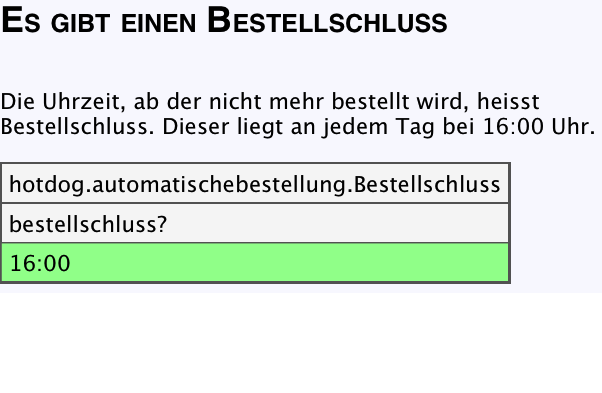
\includegraphics[width=5cm]{bestellschluss.png}
%\hfill{}
%\onslide+<2->
%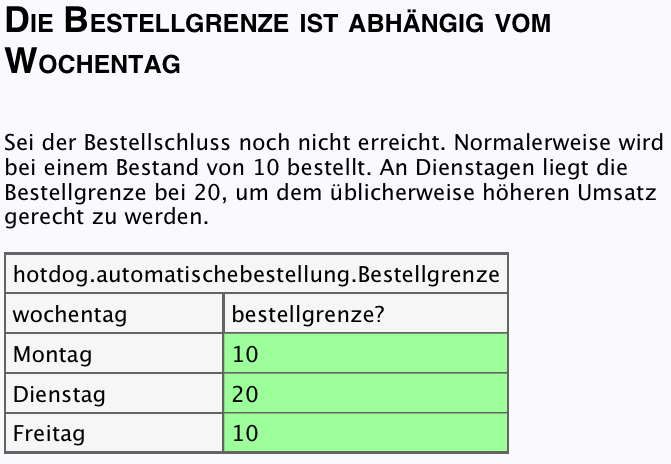
\includegraphics[width=5cm]{wochentag.png}
% \newline
%\onslide+<3->
%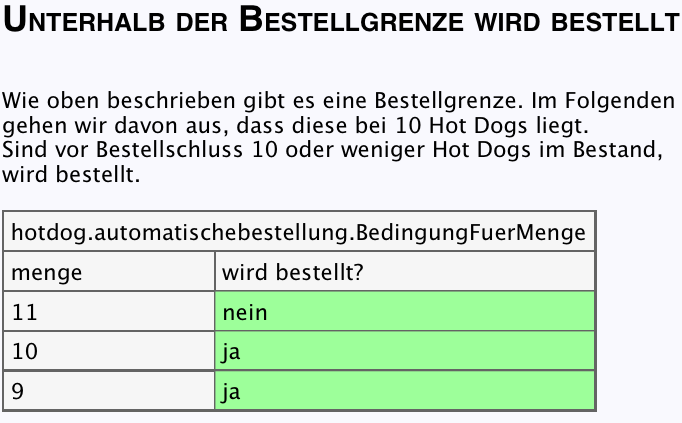
\includegraphics[width=5cm]{bestellgrenze.png}
%\hfill{}
%\onslide+<4->
%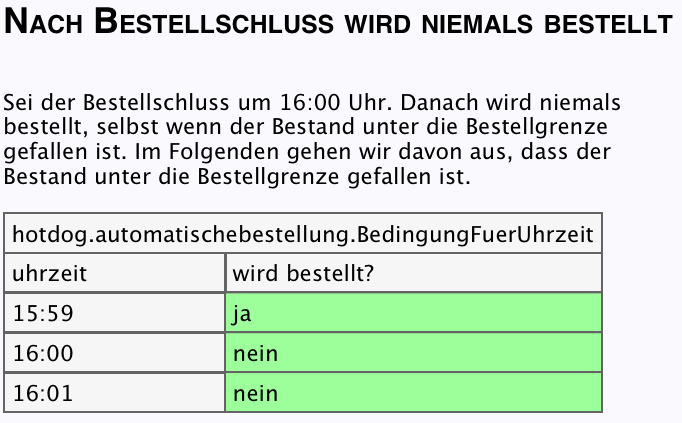
\includegraphics[width=5cm]{keineBestellungNachBestellschluss.png} 
%\end{center}

\end{frame}

%%%%%%%%%%%%%%%%%%%%%%%%%%%%%%%%%%%%%%%%%%%%%%%%%%
\begin{frame}{Fazit}

\begin{itemize}
	\item Zentraler Aspekt ist Kommunikation im Specification Workshop
	\item Wesentliche Ergebnisse:
	\begin{itemize}
		\item Eine fachliche Modellierung der Domäne
		\item Ausführbare Spezifikationsbeispiele (Tests)
	\end{itemize}
	\item Spezifikation geht alle an (Auftraggeber, Entwickler, QA, Support)
	\item Dann ist es möglich, eine Quelle für Anforderungen und Dokumentation mit Verbindung zur Anwendung zu haben
\end{itemize}

\end{frame}

%%%%%%%%%%%%%%%%%%%%%%%%%%%%%%%%%%%%%%%%%%%%%%%%%%
\begin{frame}{Bücher zum Thema}

\begin{center}
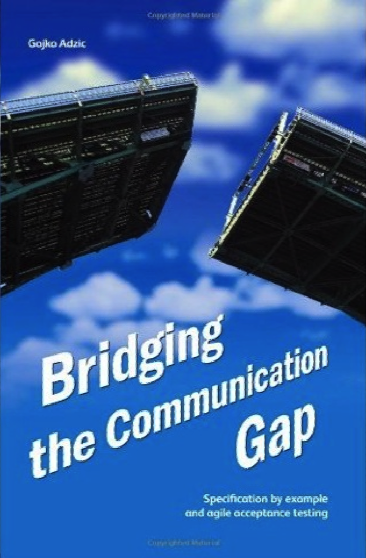
\includegraphics[height=7cm]{CommunicationGap.png}
\hfill

\includegraphics[height=7cm]{SpecificationByExample.png}
\end{center}

\end{frame}

%%%%%%%%%%%%%%%%%%%%%%%%%%%%%%%%%%%%%%%%%%%%%%%%%%
{
\usebackgroundtemplate{
\includegraphics[width=\paperwidth,height=\paperheight]{background-slide.png}}
\begin{frame}{}

\begin{center}
\Large
Vielen Dank!
\end{center}

        Folien auf GitHub:
        \vspace{-0.8em}
        \begin{center}
                \url{https://github.com/leider/Beispielhaft}
        \end{center}

        \begin{block}{Nicole Rauch}
        \begin{description}[Twitterxx]
                \item[E-Mail]  \href{mailto:info@nicole-rauch.de}{\texttt{info@nicole-rauch.de}}
                \item[Twitter] \href{http://twitter.com/NicoleRauch}{\texttt{@NicoleRauch}}
        \end{description}
        \end{block}
\end{frame}
}

%%%%%%%%%%%%%%%%%%%%%%%%%%%%%%%%%%%%%%%%%%%%%%%%%%
%\begin{frame}{Quellen}
%
%\begin{itemize}
%\item Kompliziert.jpg: 
%\url{http://chestofbooks.com/crafts/metal/Elementary-Metal-Work/Nails-And-Nailed-Strips.html}
%\item Formeln.jpg: 
%\url{http://depts.washington.edu/ecnboard/wordpress/wp-content/uploads/2011/01/math_image-300x269.jpg}
%\item Namen.jpg: 
%\end{itemize}
%
%\end{frame}
